\section{Neurona biológica}
\subsection{La neurona}
La neurona es un tipo de célula perteneciente al sistema nervioso central, que se comunica tanto por señales eléctricas como por señales químicas. Cada neurona tiene:


 \begin{itemize}
	\item Un cuerpo celular (\textbf{soma}) que contiene un núcleo y otros componentes celulares.
	\item Una zona de recepción con protuberancias elongadas denominadas \textbf{dendritas}.
	\item Una zona de emisión conocida como \textbf{axón}, el cual está compuesto de:
		\begin {itemize}
			\item Cono axónico.
			\item Membrana plasmática axónica y citoplasma.
			\item Recubrimiento de mielina, interrumpido a intervalos regulares por nódulos (anillos) de Ranvier.
			\item Terminales del axón donde se encuentan los \textbf{botones sinápticos}. 
		\end{itemize}
 \end{itemize}


\begin{figure}[h]
 \centering
 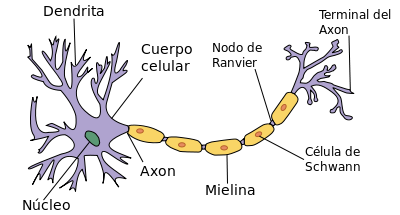
\includegraphics[scale=0.6]{../Figuras/neuronaPartes.png}
 \caption{Neurona, Acracia, 14 January 2007, Wikimedia Commons, \url{https://commons.wikimedia.org/wiki/File:Neurona.svg}, Creative Commons Attribution-ShareAlike 2.5 Generic}
 \label{fig:neuronaP}
\end{figure}


 Pensemos en la neurona como toda una compuerta, por un lado, está el cuerpo de una neurona típica, por otro lado están las dendritas y axones donde tienen lugar la mayoría de las reacciones que permiten la transmisión de información.  La forma en que fluye esta información es mediante sustancias químicas (neurotransmisores) y iones ($Na+, K+, Cl-$, etc.) que se están intercambiando entre la parte de afuera y de adentro de la neurona, a través de su membrana.
 
 Particularmente en las dendritas y axones se tienen terminaciones que se pueden conectar con otras neuronas y de esta manera permitir el paso de información. En estos puntos de conexión se indentifica a las neuronas participantes como:
 
 \begin{itemize}
  \item Neurona presináptica, transmite una señal.
  \item Neurona postináptica, recibe una señal.
 \end{itemize}  
 
La presencia de estos iones provoca que en el interior de la neurona haya una cierta carga eléctrica, mientras que en el exterior (el líquido de afuera) hay otra carga eléctrica, es decir, hay una \textbf{diferencia de potencial} entre el interior y el exterior de la neurona, por eso se dice que la membrana axónica en sí misma tiene una carga eléctrica. Dado que es porosa, esta membrana  va a estar intercambiando partículas con el exterior, esto va a hacer que su polarización varíe con el tiempo, si en algún momento la diferencia de potencial neta rebasa un cierto umbral la neurona emitirá un pulso que afectará a las neuronas con las que esté conectada.




Transmisión de señales y almacenamiento de información:


\begin{enumerate}
 \item La neurona desde sus dendritas recibe señales de otras neuronas vecinas.
 \item Cada señal se va acumulando en su cuerpo hasta el cono axónico, donde se van a estar sumando la contribución de todos los efectos de cambios de potencial.
 \item En el momento que se rebase un cierto valor umbral, la diferencia de potencial se propaga hasta los botones terminales.
 \item La neurona entra en un período refractario, donde empieza a cambiar el potencial entre el cono axónico y el axón de la neurona.
 \item Se va a transmitir un disparo eléctrico en seguida,
 \item La neurona se va a quedar totalmente quieta, durante un breve momento para que la señal pueda viajar hacia el axón.
 \item Se va a notar un cambio muy violento en el voltaje, que se va recorriendo a lo largo de todo el axón. 
\end{enumerate}


La neurona típica tiene unas células de mielina, que forman nodos que van cubriendo al axón para evitar que se pierda la señal, estos nodos recargan la señal permitiendo que avance al siguiente nodo, donde se recarga nuevamente y avanza, hasta que logra llegar al final de axón.


\begin{figure}[h]
 \centering
 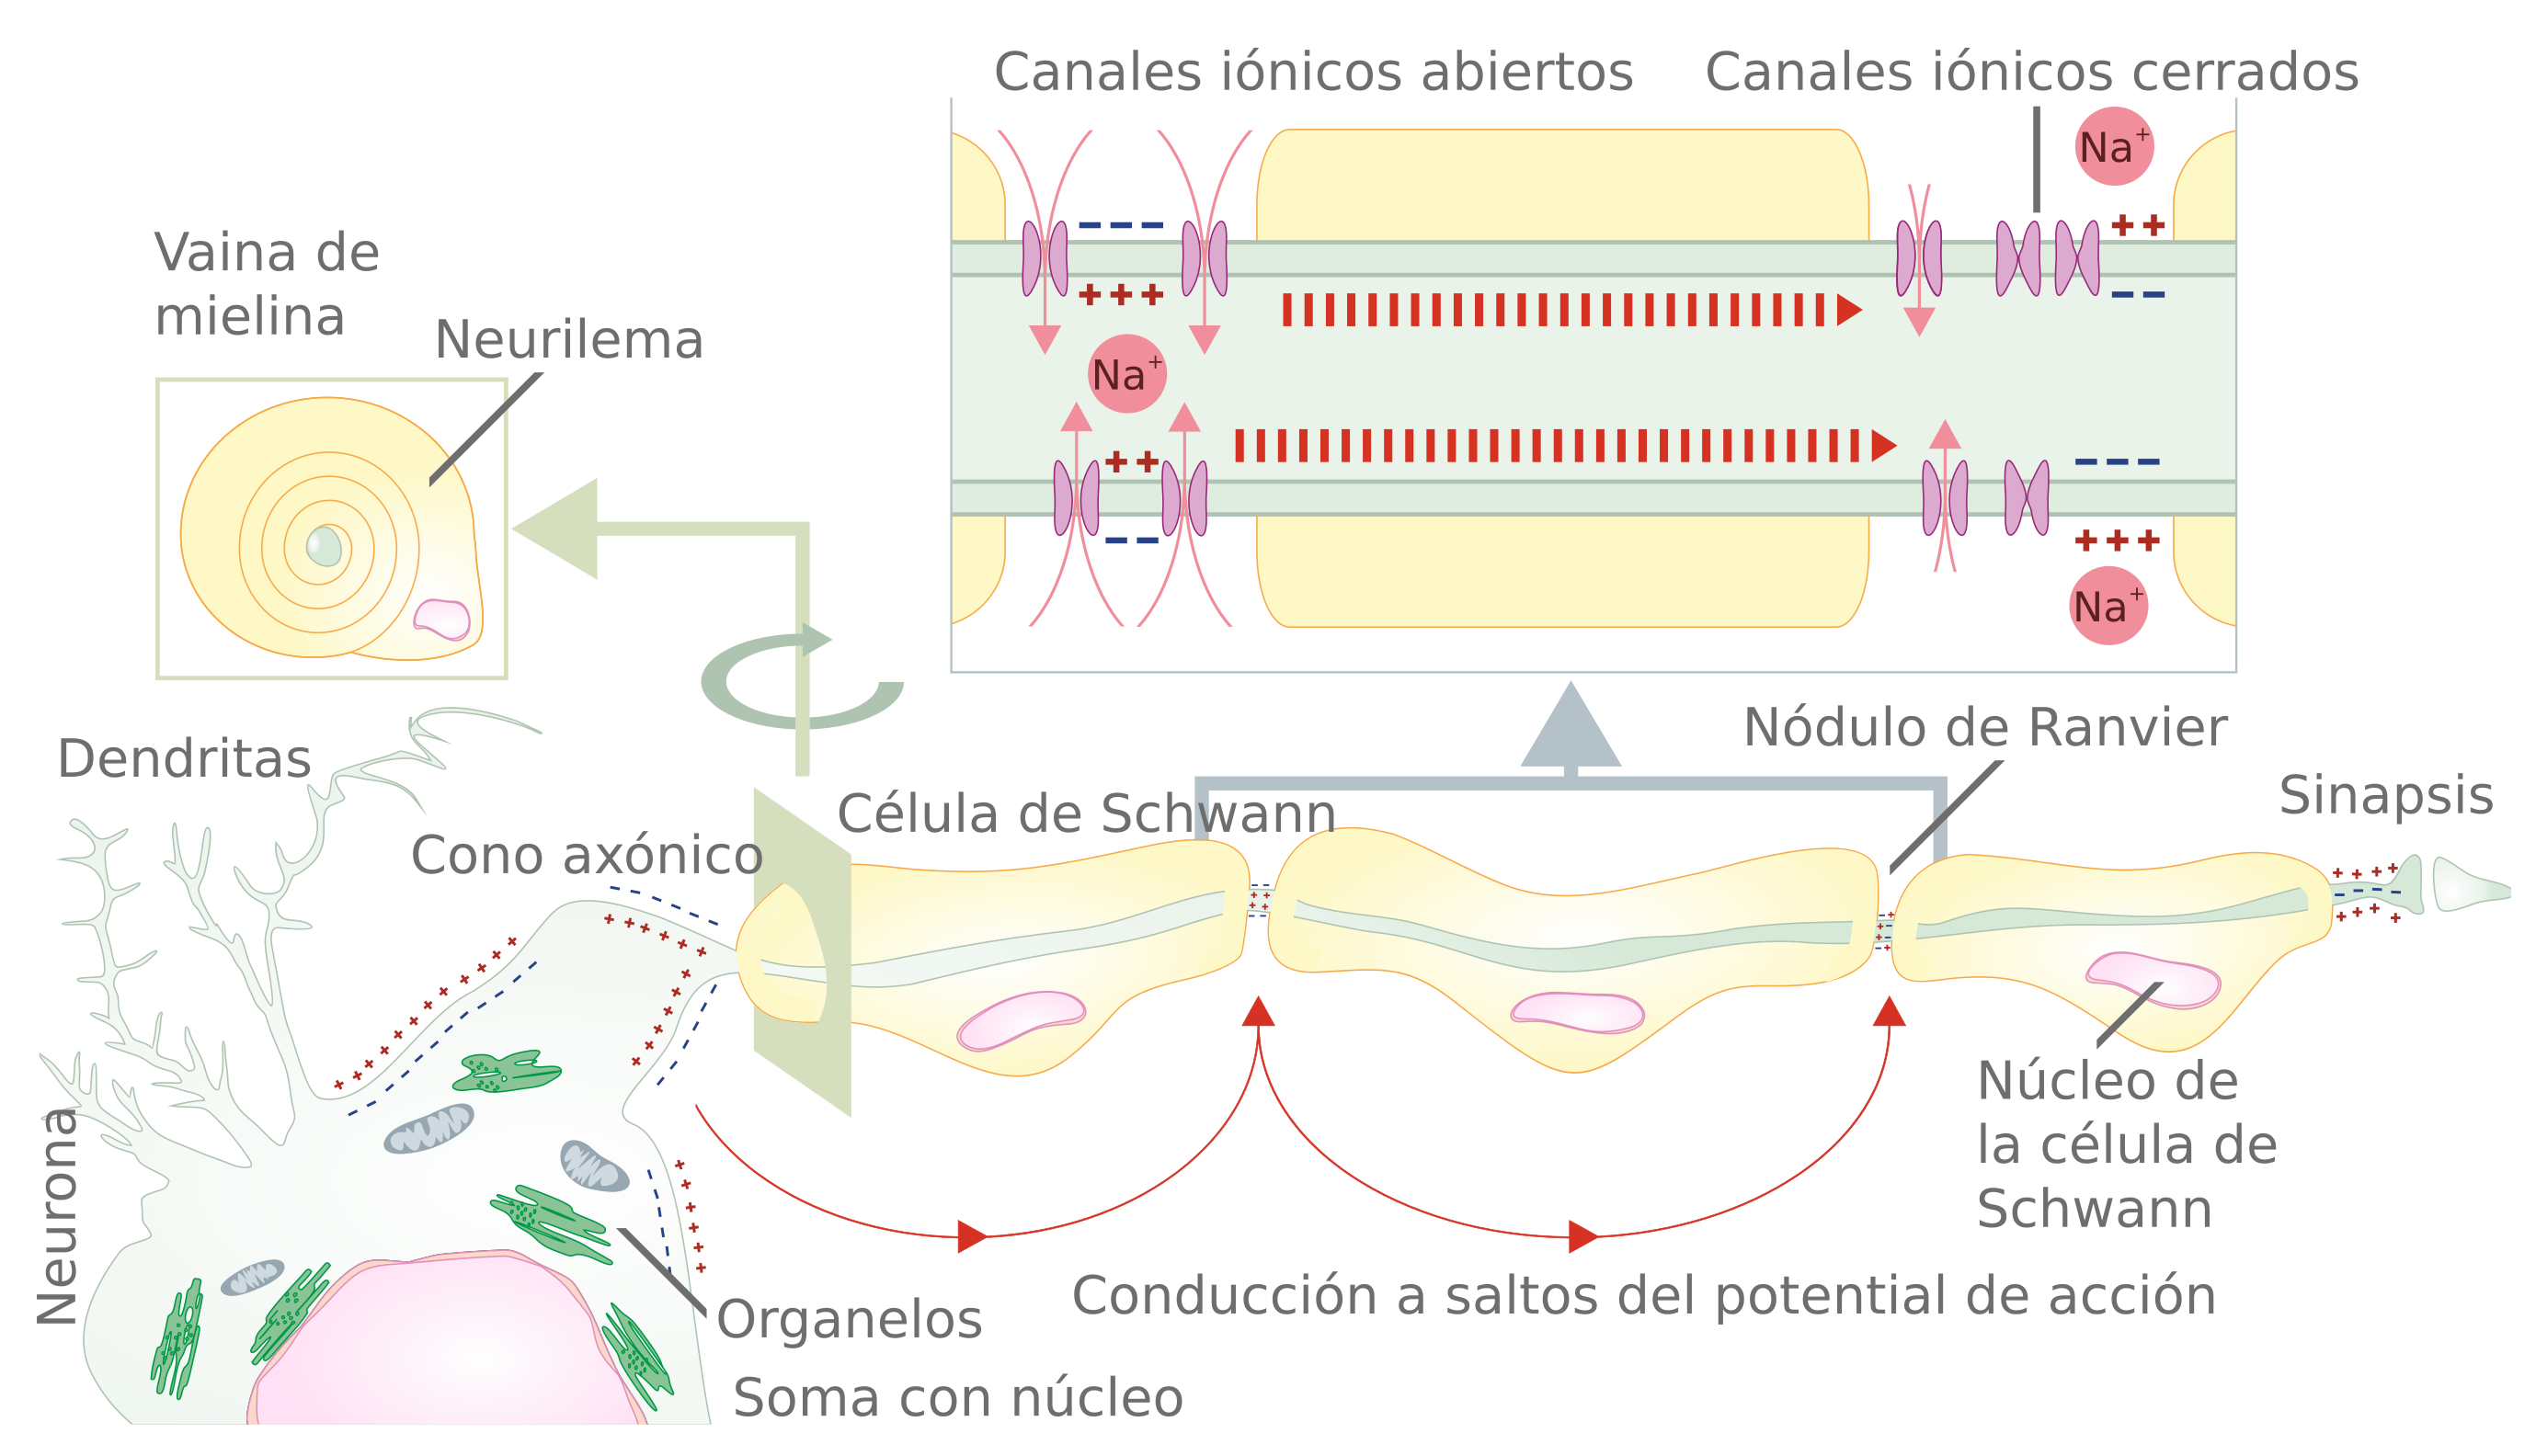
\includegraphics[scale=0.1]{../Figuras/Saltos.png}
 \caption{Corriente iónica por el axón (efecto de corto plazo), Helixitta, 1 octubre 2015, Wikimedia Commons, \url{https://commons.wikimedia.org/wiki/File:Propagation_of_action_potential_along_myelinated_nerve_fiber_en.svg}, Creative Commons Attribution-ShareAlike 4.0 International}
 \label{fig:conduccionSaltos}
\end{figure}


Este trayecto puede ser de una neurona a unas pocas neuronas vecinas, hasta unos cuantos metros (ej. esta podría estar en la médula espinal y el axón llegar hasta el dedo del pie). Cuando la señal llega a la terminal del axón, hay varias terminales que van a reaccionar ante el cambio de electricidad mediante la liberación de unas vesículas, que contienen \textbf{neurotransmisores}.




\subsection{Elementos de las neuronas y tipos}


Elementos que participan durante la transmisión de señales:


\begin{itemize}
\item \textbf{Impulsos eléctricos:} potenciales de acción que son, cambios de voltaje que van a ir ocurriendo a lo largo del axón. Sucede una vez que se acumularon demasiadas señales a través de las dendritas, entonces la neurona puede disparar un impulso eléctrico, a través del axón, que va a provocar que su terminal libere más químicos, estos químicos son los que hacen los efectos pequeños en cada uno de los cuerpos de las neuronas postsinápticas.

\item \textbf{Neurotransmisores:} son los mensajeros químicos que se comunican entre neuronas adyacentes. La liberación de neurotransmisores de una neurona ayudará a despolarizar o hiperpolarizar (aumentar la magnitud de la carga) de la neurona adyacente, lo que hará que sea más o menos probable que ocurra un potencial de acción en la siguiente neurona.
 
\item \textbf{Plasticidad:} modificación a largo plazo de las conexiones entre neuronas. En el cerebro las neuronas pueden cambiar de manera permanente, perder canales (que permiten el intercambio de nuevos transmisores sin impulsos eléctricos), formar más canales o incluso pueden crear protuberancias. Cuando un cerebro aprende está transformando su arquitectura, es decir, los aprendizajes de largo plazo modifican el cerebro y en consecuencia va a pensar y reaccionar distinto que antes del aprendizaje.
\end{itemize}




Clasificación de tipos de neuronas:


\begin{figure}[h]
 \centering
 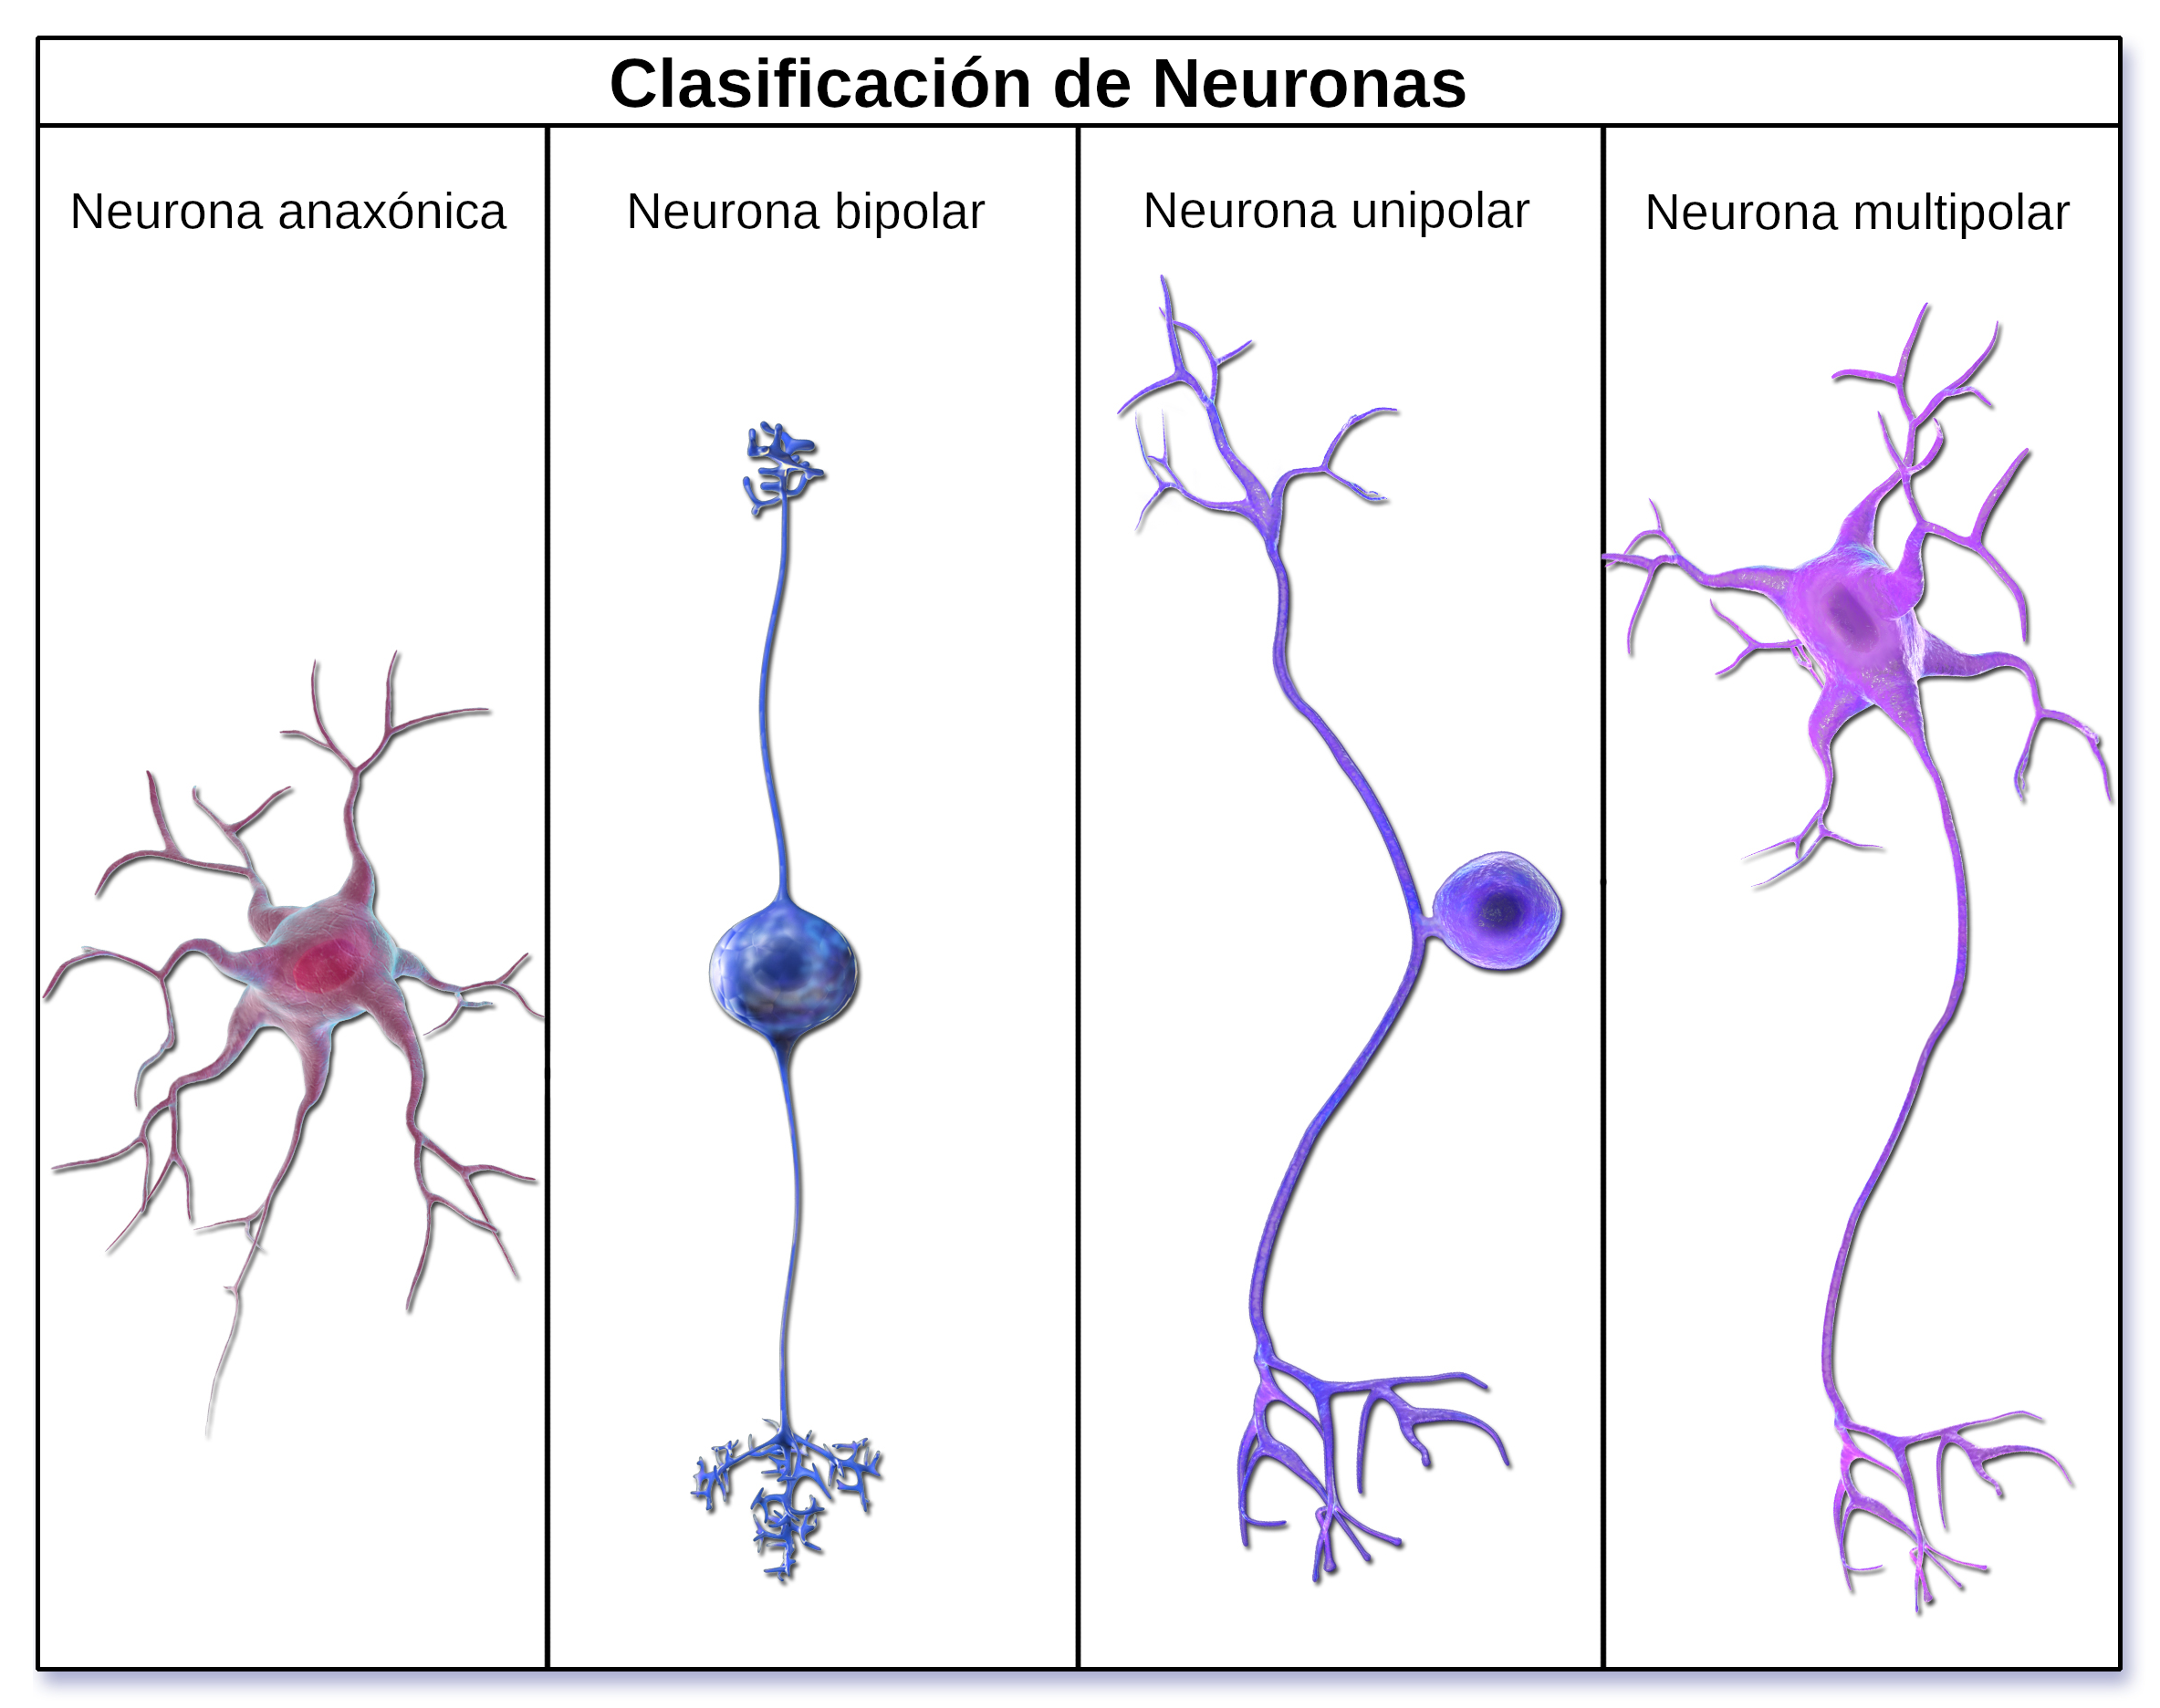
\includegraphics[scale=0.15]{../Figuras/tiposDeNeuronas.png}
 \caption{Representación de la clasificación de neuronas, BruceBlaus, 26 junio 2017, Wikimedia Commons, \url{https://commons.wikimedia.org/wiki/File:Neuron_Classification.png}, Creative Commons Attribution-ShareAlike 4.0 International}
 \label{fig:tiposNeuro}
\end{figure}




\begin{itemize}
\item \textbf{Neurona sin axones}, nunca dispara, pero sí tiene intercambios de neurotransmisores en las dendritas 
\item \textbf{Neurona bipolar}, tiene dos axones. 
\item \textbf{Neurona unipolar}, solamente hay una conexión entre el cuerpo y el axón, pero el axón tiene dos ramas, cuando dispare va a disparar hacia los dos lados, haciendo llegar su señal a diferentes regiones. 
\item \textbf{Neurona multipolar}, la más conocida, empieza con un cuerpo con dendritas y luego un largo axón que va a terminar con varias terminaciones axónicas. 
\end{itemize}


Cuando modelamos redes neuronales lo típico es modelar una neurona con dendritas, su disparo y su axón, que se conecta con las dendritas de las siguientes neuronas, pero aquí ya estamos viendo que la naturaleza nos dice que hay que pensar más y plantear cómo hacer las representaciones de estas conexiones que nos presenta la naturaleza, un poco diferente pero tal vez con resultados más satisfactorios.




\subsection{Sinapsis}


Aquí veremos más a detalle cómo una neurona recibe o transmite información a otras neuronas, donde para un solo disparo están participando un montón de elementos que veremos más adelante.


 El momento en que dos neuronas transmiten información se llama \textbf{sinapsis} y es mediante conexiones que se dan en las terminales del axón (vesículas sinápticas) de la neurona presináptica hacia la postsináptica. Es importante notar que estas neuronas no tienen contacto anatómico, sino que están separadas por un espacio muy pequeño, \textbf{la brecha sináptica}. Lo que sucede en estas conexiones es un intercambio electroquímico que produce cambios de polaridad a lo largo la membrana. 




\begin{figure}[h]
 \centering
 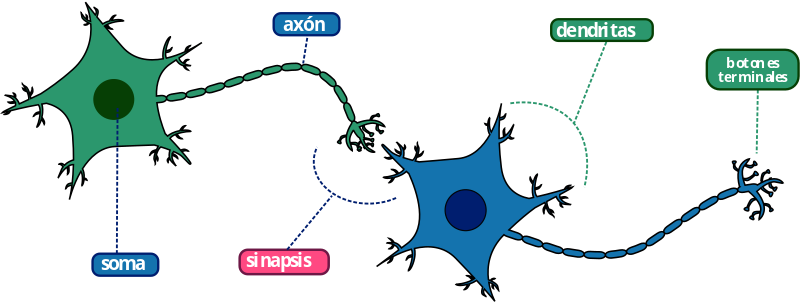
\includegraphics[scale=0.5]{../Figuras/Part_of_neurons_in_Spanish.png}
 \caption{Part of neurons in Spanish, Dana Scarinci Zabaleta, 24 febrero 2019, Wikimedia Commons, \url{https://commons.wikimedia.org/wiki/File:Part_of_neurons_in_Spanish.svg}, OpenStax, CC0}
 \label{fig:sinapsisN}
\end{figure}


Clasificación de sinapsis, las terminales del axón de la neurona presináptica puede hacer contacto con la neurona postsináptica en:
\begin{enumerate}
 \item su dendritas, axodendrítica.
 \item su cuerpo (soma), axosomática. 
 \item su axón, axoaxónica.
\end{enumerate}


Distingamos entre dos tipos de sinapsis:


 \textbf{Sinapsis eléctrica:} las membranas de las células pre y posinápticas se unen en la brecha sináptica por una unión tipo gap, o unión comunicante, que son pequeños canales que permiten el paso de iones.


	\begin{enumerate}
  	 \item Posee una transmisión bidireccional de los potenciales de acción.
  	 \item Sincronización en la actividad neuronal, lo cual hace posible una acción coordinada.
 	 \item Los potenciales de acción pasan a través del canal proteico directamente sin necesidad de la liberación de los neurotransmisores, por tanto, es más rápida.
	\end{enumerate}


\begin{figure}[h]
 \centering
 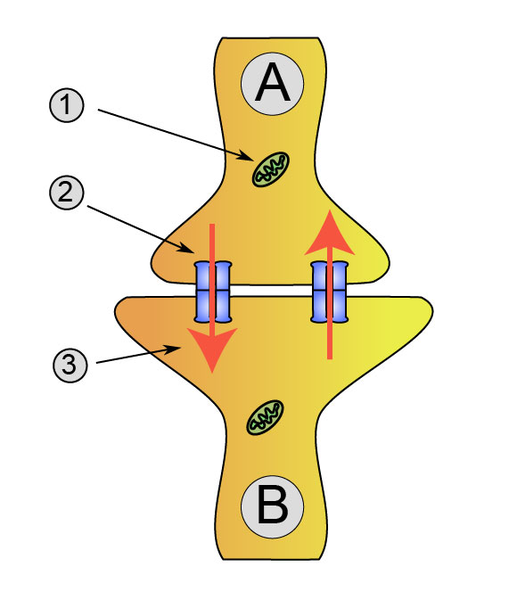
\includegraphics[scale=0.4]{../Figuras/sinapsisElectrica.png}
 \caption{Synaptical transmission (electrical). Neurona A transmisora, Neurona B receptora, 1. Mitocondria, 2. Uniones gap formadas por conexinas, 3. Señal eléctrica, Nrets~commonswiki, 23 September 2005, Wikimedia Commons, \url{https://commons.wikimedia.org/wiki/File:Synapse_diag2.png}, Inkscape 0.42, CC-BY-SA 3.0}
 \label{fig:sinapsisN}
\end{figure}
 
 \textbf{Sinapsis química:} la neurona libera moléculas neurotransmisoras a otra neurona adyacente en un pequeño espacio (la brecha sináptica) ver \ref{fig:sinapsisQ}. Se puede resumir en cuatro etapas principales:


\begin{enumerate}
 \item Un potencial de acción llega al botón terminal proveniente desde cono axónico.
 \item Los neurotransmisores contenidos en las vesículas que están él los botones terminales, son liberados en la brecha sináptica y se dispersan.
 \item Cada neurotransmisor se une a su receptor ubicado en la membrana de la neurona postsináptica.
 \item El exceso de neurotransmisores que queda en el espacio sináptico es degradado o recaptado.
\end{enumerate}


\begin{figure}[h]
 \centering
 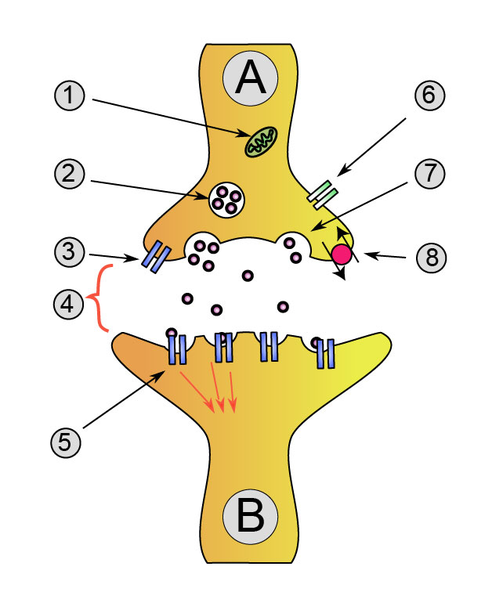
\includegraphics[scale=0.4]{../Figuras/SinapsisQuimica1.png}
 \caption{Synaptical transmission (chemical). Neurona A transmisora, Neurona B receptora, 1. Mitocondria, 2. Vesícula sináptica llena de neurotransmisor, 3. Autorreceptor, 4. Brecha sináptica, 5. Receptor de neurotransmisores, 6. Canal de calcio, 7. Neurotransmisor liberador de vesículas fusionadas, 8. Bomba de recaptación de neurotransmisores, Utilisateur:Dake, 23 September 2005, Wikimedia Commons, \url{https://commons.wikimedia.org/wiki/File:Synapse_diag1.png}, Inkscape 0.42, CC-BY-SA 3.0}
 \label{fig:sinapsisQ}
\end{figure}




Detallando el proceso de la sinapsis química, la neurona postsináptica está recibiendo un montón de señales por la liberación de neurotransmisores tanto de sus vecinos, como lo que ella misma va intercambiando, una vez que están generando el efecto completo de cambiar la polarización de la membrana, van a provocar que la neurona haga un disparo eléctrico. En el cuerpo están llegando estos intercambios de iones que se suman en el cono axónico, empiezan a viajar a través del axón, en las vainas de mielina (donde se refuerza la señal). 
Aquí hacemos mención por primera vez de los iones positivos: sodio y potasio, estos iones lo que hacen es, que \emph{la membrana tenga una cierta carga la mayor parte del tiempo}. Cuando salen tres sodios entran dos potasios, entonces siempre hay más positivos afuera que en el interior de la neurona, es decir, por lo general  \emph{tiene una carga más negativa que su entorno} (ver \ref{fig:MembranaP}). Cuando ocurre un disparo de la neurona y se da el cambio de polarización en la membrana, se abren sus poros/ canales. El hecho que los canales abran o cierren depende de varios cambios que puedan estar ocurriendo alrededor de la neurona, en particular los que transmiten el disparo eléctrico, reaccionan ante el cambio de potencial que ocurrió en la membrana de la neurona. 


La señal va pasando por los nodos de Rainvier, se refuerza y pasa por los canales iónicos ya abiertos, hasta finalmente llegar a la sinapsis a esto le llaman la \textbf{conducción a saltos} (ver \ref{fig:conduccionSaltos}). Ahora lo que ocurre al final del recorrido es que, el cambio de electricidad otra vez provoca que unas vesículas, que están en el interior de la neurona, que contienen neurotransmisores, se peguen a la membrana axónica y se liberen esos neurotransmisores nuevamente a otra neurona. 


Entonces la información le va a llegar a la neurona vecina, en la forma de neurotransmisores que fueron liberados (en lo que sea que lo haya recibido, típicamente son dendritas, pero podría ser su cuerpo o su axón), eso es lo que va a percibir la otra neurona y otra vez esta otra neurona va a empezar a sumar los efectos de estos neurotransmisores, para que en algún momento decida a lo mejor disparar y otra vez provocar que se liberen neurotransmisores a su final e influir con otras neuronas.


\subsubsection{Neurotransmisón}
Cuando la neurona no está mandando señales eléctricas, tiene un potencial de reposo, su diferencia de potencial entre el interior y el exterior de la neurona, es más negativo en el interior y más positivo (o menos negativo) en el exterior.
En el caso de las sinapsis químicas, llega un disparo y se altera el potencial de la membrana, entrarán las
células de calcio y entra la participación de las vesículas para liberar neurotransmisores. Los neurotransmisores están flotando en la brecha sináptica, viajan hasta adherirse a los receptores de la neurona posináptica, en ese momento están alterando el intercambio normal que existe entre \underline{iones en el interior y en el exterior} de la célula y van a cambiar las cargas netas que hay adentro y afuera. Este es un cambio local que está ocurriendo en las  espinas dendríticas (pequeñas prolongaciones citoplasmáticas).


\begin{figure}[h]
 \centering
 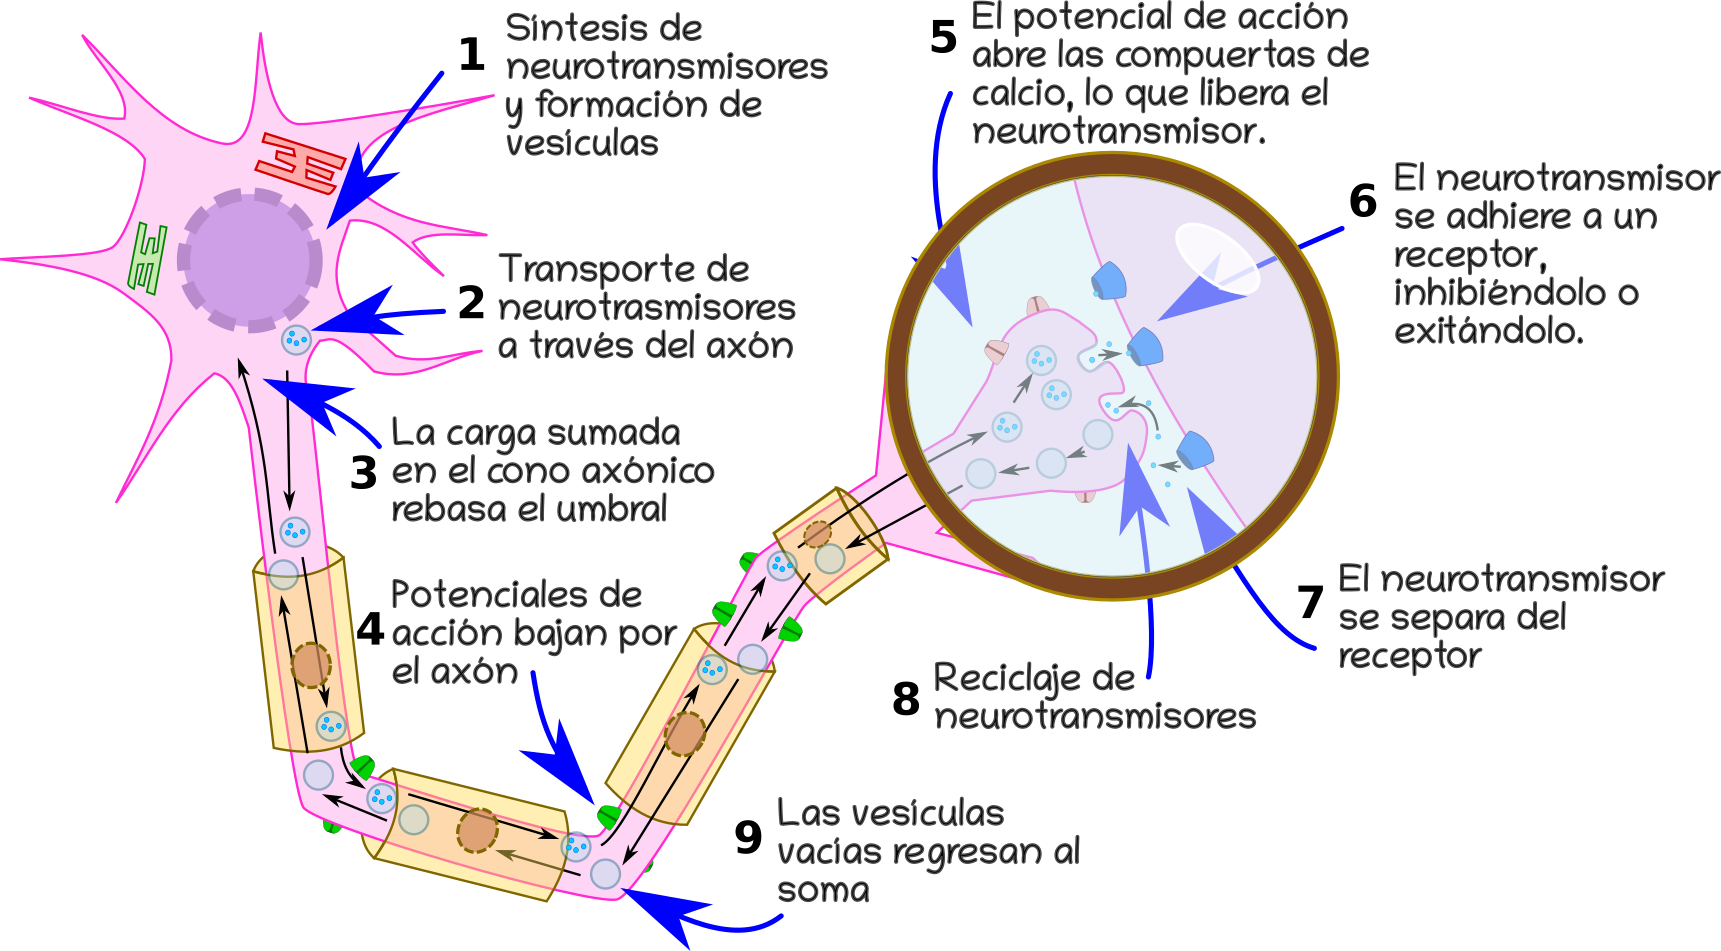
\includegraphics[scale=0.2]{../Figuras/neurotransmision.png} 
 \caption{Esquema detallado de una neurotransmisión.}
 \label{fig:nTransmision}
\end{figure}


este cambio en sí es una especie de transferencia de información, pero muy local.Se puede distinguir entre dos efectos en la membrana: 


\begin{itemize}
\item \textbf{El efecto excitatorio}, despolariza la membrana postsináptica es decir ahora va a ser más propensa a disparar porque ya le cambió la diferencia de potencial que tenía.  
\item \textbf{El efecto inhibitorio}, hiperpolariza la membrana postsináptica, es decir, va a incrementar la diferencia de potencial entre el exterior e interior, pero de tal manera que ahora ya no va a querer disparar esta neurona.
\end{itemize}


De estos efectos también va a darse el efecto de la \textbf{plasticidad}, que es cuando dos neuronas tienden a excitarse juntas, después de esta conexión se va a tender fortalecer, sí más bien tienden a inhibirse lo que va a suceder después es que estos canales empiezan a encoger, haciendo que se reduzcan y ya no dispare.


Ejemplos de neurotransmisores: serotonina, dopamina, oxitocina, endorfinas, adrenalina.




\subsection{Campos receptivos}
Aquí lo que nos interesa es, en qué región puede ser afectada una neurona. Se define un campo receptivo, como la región en la periferia sensorial
dentro de la cual los estímulos pueden, influir la actividad de las células sensoriales (ver \ref{fig:camposR}). Hay diferentes niveles donde pueden aparecer los campos receptivos tanto cerca de la piel, cerca del gusto, el olfato, donde las neuronas van a estar asociadas con otras células que les pueden ayudar, que son sensitivas a los cambios correspondientes, a veces la misma neurona va a tener alguna protuberancia especializada.
También podemos encontrarlos más hacia adentro del nivel de procesamiento, no necesariamente todos van a estar pegados a la parte sensorial física. 
\begin{figure}[h]
 \centering
 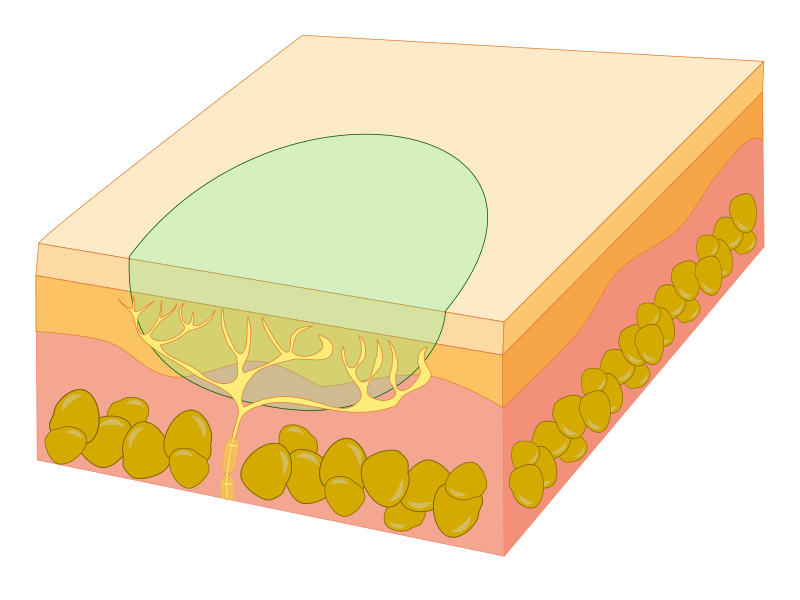
\includegraphics[scale=0.3]{../Figuras/camposreceptores.png}
 \caption{Campo receptivo. Se muestra una región que está bajo cierto estímulo, las terminales de la neurona está recibiendo está información y transmitiéndola.}
 \label{fig:camposR}
\end{figure}


Comprenden a los receptores sensoriales que alimentan a las neuronas sensoriales, pueden ser:


\begin{itemize}
\item Receptores específicos en una neurona como protuberancias especializadas. 
\item Conjuntos de receptores capaces de activar una neurona mediante conexiones sinápticas. 
\item Describen la ubicación donde debe estar presente un estímulo sensorial para licitar una respuesta desde una célula sensorial. 
\end{itemize}


Ejemplos:


\begin{itemize}
\item En la piel tenemos células que nos están protegiendo en la epidermis, una de las células auxiliares \textbf{la célula de Merkel} que es
sensible a la presión. Esta puede estar muy cerca a una neurona, sus terminales se activan de acuerdo a las acciones de la célula de Merkel y va a pasar la información (ver \ref{fig:mer}).  
 	
\begin{figure}[h]
 \centering
 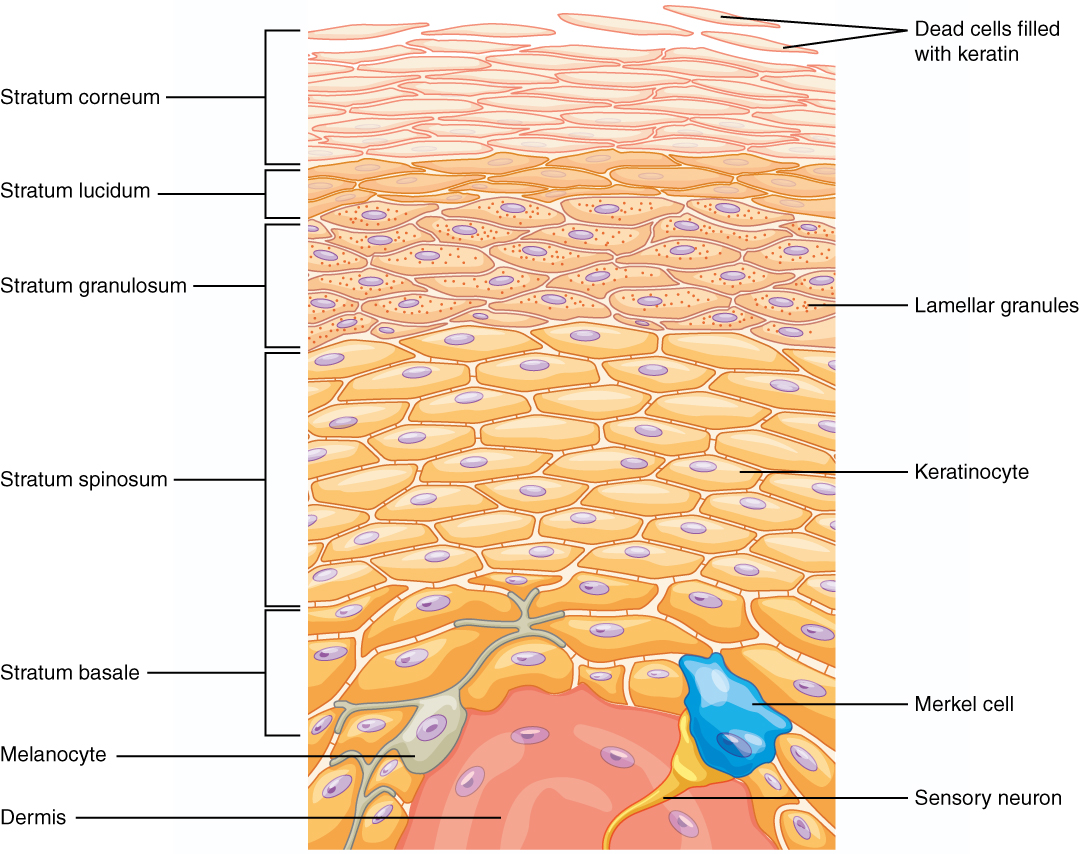
\includegraphics[scale=0.2]{../Figuras/merkel.png}
 \caption{Capas de la epidermis y en azul la célula de Merkel.}
 \label{fig:mer}
\end{figure}


\item El ojo, para procesamiento visual, actualmente se utiliza una de las redes neuronales más famosas que son las redes convolucionales, que están inspiradas en el ojo, nosotros tenemos campos receptores donde hay unos fotorreceptores en los conos y los bastones que son sensibles a luces de diferentes colores a cambios de intensidad de la luz y que pueden detectar, por ejemplo, en una cierta región física si está llegando luz  o por ejemplo, si llega en la periferia entonces va a inhibir el disparo de estos elementos, por otro lado, tenemos también su complemento que permite ser estimulado por las señales que llegan, como que en la parte de afuera de un círculo y más bien se inhiben con un estímulo en la parte de afuera (ver \ref{fig:nSen}). Esta especie de celdas que tienen una posición física y geométrica relevante van a determinar cuando disparan o no las neuronas. Los siguientes niveles del cerebro se van a encargar de interpretar mejor  el cambio de sombras, como a una persona que pasó corriendo, un auto que se está moviendo cerca o reconocer algún tipo de alimento.
\end{itemize}


\begin{figure}[h]
 \centering
 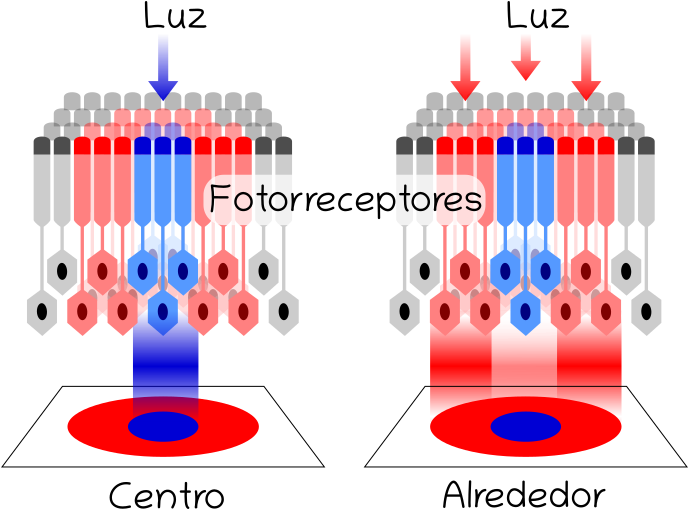
\includegraphics[scale=0.5]{../Figuras/nSensitivas.png}
 \caption{Capas de la epidermis y en azul la célula de Merkel.}
 \label{fig:nSen}
\end{figure}




\subsection{Señal eléctrica}
Veamos que pasa en los canales de iones y el paso de la señal eléctrica primero diferenciemos los tipos de compuertas iónicas:


\begin{itemize}
\item \textbf{Canal por fuga:} Estos se abren y cierran aleatoriamente, todo el tiempo están activos en la neurona, intercambiando por ejemplo: sodio y potasio.
\item \textbf{Canal regulado por ligado:} Aquí se hace presente un neurotransmisor que es el que va a provocar que se abran o al revés impedir que se abran.
\item  \textbf{Canal por estímulo mecánico:} Permiten que pasen más iones o menos iones dependiendo, si se ejerció una presión, por ejemplo, con las neuronas cerca
de la piel, las células de merkel.
\item \textbf{Canales regulados por el voltaje:} Tienen el rol protagónico en la transmisión del pulso eléctrico (que se ha estado mencionando) describiendo uno de ellos, este canal tiene una pequeña compuerta abajo, que la puede cerrar independientemente del hecho de que el canal se abre o se cierre. Existen varias variantes de este tipo de canales regulados por el voltaje, la forma en que se están activando y desactivando sus compuertas, es lo que permite el paso del pulso.
\end{itemize}


Existen realmente una buena cantidad de iones presentes en el cerebro, pero los más protagónicos son precisamente el \textbf{potasio}, el \textbf{sodio}, el \textbf{cloro} y son los que vamos a utilizar para un modelo matemático de las neuronas. 


\begin{figure}[h]
 \centering
 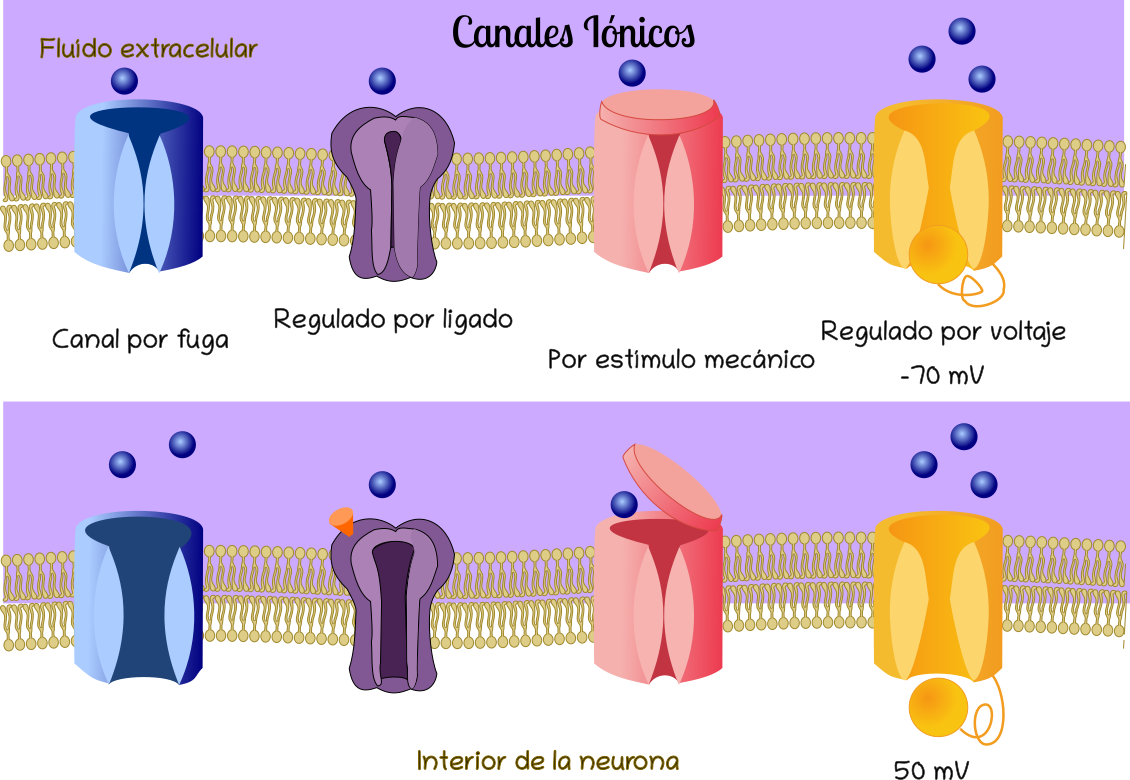
\includegraphics[scale=0.28]{../Figuras/canalesIonicos.png}
 \caption{Representación de la clasificación de los canales iónicos (más representativos).}
 \label{fig:MembranaP}
\end{figure}




Por último veamos brevemente \textbf{la neuroplasticidad}, es lo que nos permite el aprendizaje a largo plazo en el cerebro, es un mecanismo de aprendizaje del cerebro en el cual:


Cuando las neuronas se activan simultáneamente con frecuencia la conexión entre ellas se fortalece.


Este mecanismo constituye la principal inspiración para el diseño de las redes neuronales artificiales, concretamente en esto se inspiran los algoritmos de entrenamiento. Lo que se hace es calcular, qué conexiones debemos reforzar y cuáles debemos de debilitar para que nuestras redes neuronales calculen las funciones que a nosotros nos interesan.


\begin{figure}[h]
 \centering
 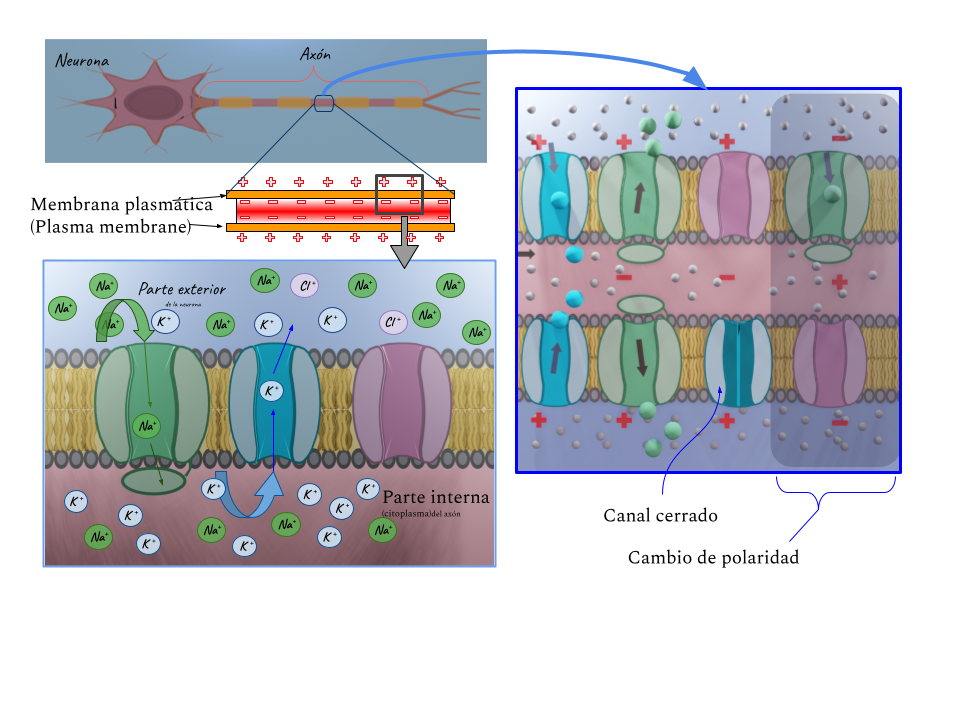
\includegraphics[scale=0.5]{../Figuras/MembranaP.png}
 \caption{Representación de la membrana axónica en potencial de reposo en la parte infererior izquierda, y en la parte derecha con un estímulo que genera el cambio de polaridad en la misma, así como el cierre de canales y paso de iones.}
 \label{fig:MembranaP}
\end{figure}


